%Version 3.1 December 2024
% See section 11 of the User Manual for version history
%
%%%%%%%%%%%%%%%%%%%%%%%%%%%%%%%%%%%%%%%%%%%%%%%%%%%%%%%%%%%%%%%%%%%%%%
%%                                                                 %%
%% Please do not use \input{...} to include other tex files.       %%
%% Submit your LaTeX manuscript as one .tex document.              %%
%%                                                                 %%
%% All additional figures and files should be attached             %%
%% separately and not embedded in the \TeX\ document itself.       %%
%%                                                                 %%
%%%%%%%%%%%%%%%%%%%%%%%%%%%%%%%%%%%%%%%%%%%%%%%%%%%%%%%%%%%%%%%%%%%%%

\documentclass[pdflatex,sn-mathphys-num]{sn-jnl}

%%%% Standard Packages
\usepackage{graphicx}%
\usepackage{multirow}%
\usepackage{amsmath,amssymb,amsfonts}%
\usepackage{amsthm}%
\usepackage{mathrsfs}%
\usepackage[title]{appendix}%
\usepackage{xcolor}%
\usepackage{textcomp}%
\usepackage{manyfoot}%
\usepackage{algorithm}%
\usepackage{algorithmicx}%
\usepackage{algpseudocode}%
\usepackage{listings}%
\usepackage{tikz}%
\usepackage{url}%
\usepackage{tabularray}%

\lstset{
  basicstyle=\ttfamily\footnotesize,
  breaklines=true,
  frame=single,
  numbers=left,
  numberstyle=\tiny,
  tabsize=2,
  keywordstyle=\bfseries,
}

\raggedbottom

\begin{document}

\title[Surfacing Personal Belief Change from Digital Traces]{``I Used to Think That'': Surfacing Personal Belief Change from Digital Traces via Contradiction Detection}

\author*[1]{\fnm{Tushar} \sur{Laad}}\email{tushar@memrylab.com}

\affil*[1]{\orgname{Independent Researcher}}

\abstract{People accumulate vast personal writing across social media, journals, and messaging platforms, yet no tool helps them understand how their beliefs have changed. We present MemryLab, a privacy-preserving system that extracts structured beliefs from heterogeneous digital archives, detects temporal contradictions between them, and synthesizes second-person evolution narratives grounded in the user's own words. The core technical contribution is an efficient contradiction detection method that reduces the quadratic LLM verification cost of naive pairwise comparison: the method embeds all beliefs (linear cost), filters candidates by cosine similarity, and submits only the top-20 candidate pairs to an LLM for verification, cutting model calls by over 95 percent while maintaining F1 scores of 0.76 to 0.90 across three backends. A longitudinal case study over 14653 documents and a lightweight user study with six participants provide initial evidence that the system surfaces instances of belief evolution users had not previously articulated. MemryLab is implemented as a 4.7 MB Tauri 2.0 desktop application and runs entirely on-device across nine LLM inference backends.}

\keywords{belief evolution \and contradiction detection \and personal knowledge management \and digital footprint analysis \and retrieval-augmented generation \and privacy-preserving AI}

\maketitle

%% ===================================================================
%% 1  INTRODUCTION
%% ===================================================================
\section{Introduction}\label{sec:intro}

The average internet user maintains accounts on more than eight social media platforms \cite{datareportal2024} and generates thousands of messages, posts, and journal entries each year. Under GDPR \cite{gdpr2016} and similar regulations, individuals can now download comprehensive archives of this activity. Yet no tool helps people answer a deceptively simple question: \emph{how has my thinking changed?}

Existing personal information management systems \cite{jones2007pim,lansdale1988psychology} and digital memory tools such as MyLifeBits \cite{gemmell2002mylifebits} and Microsoft Recall \cite{microsoft2024recall} treat documents as independent retrieval targets. They answer ``what did I write?'' but not ``how have my beliefs evolved?'' Consider a person who in 2019 journaled ``I value stability above all else'' and by 2023 was posting about embracing uncertainty. This belief shift is invisible to any retrieval system, yet it is precisely the kind of self-knowledge that supports reflection and growth.

We term this the \emph{meta-narrative problem}: understanding not just what one wrote, but how one's thinking has changed. Addressing it requires (1)~ingesting heterogeneous multi-platform archives, (2)~extracting structured beliefs from unstructured text, (3)~detecting temporal contradictions between beliefs, and (4)~synthesizing intelligible evolution narratives. We investigate whether a computational system can surface instances of belief evolution from personal data, and whether doing so leads users to genuine self-insight. We focus specifically on contradiction detection as a tractable and high-signal proxy for belief change.

Modern LLMs create a new opportunity: they can extract nuanced beliefs and generate coherent narratives zero-shot \cite{brown2020gpt3,touvron2023llama} without task-specific training. However, applying LLMs to the belief-evolution problem naively is computationally prohibitive---pairwise contradiction checking across $n$ beliefs requires $O(n^2)$ LLM calls---and raises acute privacy concerns that preclude cloud-only solutions.

We present MemryLab with three contributions:

\begin{enumerate}
    \item \textbf{A belief representation} modeling personal beliefs as temporally-grounded, extractable \texttt{MemoryFact} records extracted from 33 platform adapters, enabling computational analysis of how thinking shifts over time.
    \item \textbf{An efficient contradiction detection algorithm} combining embedding-based semantic pre-filtering with bounded LLM verification, reducing verification calls from $O(n^2)$ to $O(k)$ where $k \leq 20$.
    \item \textbf{Empirical evaluation} including a longitudinal case study across 14,653 personal documents and a lightweight user study ($n{=}6$) measuring insight novelty, contradiction accuracy, and narrative quality.
\end{enumerate}

%% ===================================================================
%% 2  RELATED WORK
%% ===================================================================
\section{Related Work}\label{sec:related}

\subsection{Personal Information Management and Digital Memory}

The vision of personal memory augmentation dates to Bush's Memex \cite{bush1945memex}. Bell's MyLifeBits \cite{gemmell2002mylifebits,bell2009total} demonstrated comprehensive life capture but focused on storage rather than evolution analysis. Boardman and Sasse \cite{boardman2004stuff} identified cross-tool fragmentation as a barrier to coherence; Whittaker \cite{whittaker2011personal} showed people maintain separate organizational schemes across tools. Personal knowledge graphs \cite{balog2019personal,kejriwal2021knowledge} and temporal knowledge graphs \cite{jiang2024tkg_survey,leblay2018temporal} provide formal frameworks for organizing personal information over time. What these systems share is a focus on \emph{retrieval}---none model belief \emph{change} or detect evolution. MemryLab treats documents not as retrieval targets but as evidence of mental state over time.

\subsection{Memory-Augmented AI Systems}

Recent work on persistent AI memory includes Mem0 \cite{chhikara2025mem0}, which introduces a self-improving memory layer; MemoRAG \cite{qian2025memorag}, which uses global corpus memory to improve retrieval; NEMORI \cite{nan2025nemori}, with self-organizing memory hierarchies inspired by cognitive science; Hindsight \cite{latimer2025hindsight}, which formalizes opinion evolution in agent networks; and episodic memory for RAG \cite{nair2025episodic}. These systems model what an AI agent knows, not how a \emph{user's} beliefs change across time. Xu et al.\ \cite{xu2024knowledge} survey knowledge conflicts in LLMs; we apply a related contradiction formulation to the intra-personal setting, where both conflicting facts originate from the same person at different times.

\subsection{Digital Footprint Analysis and Privacy}

Kosinski et al.\ \cite{kosinski2013private} and Youyou et al.\ \cite{youyou2015computer} showed that digital footprints contain rich psychological signals. Temporal sentiment analysis detects mood patterns \cite{thelwall2012sentiment,golder2011diurnal}, life events \cite{li2014major}, and mental health indicators \cite{de2013social}. However, this work analyzes single platforms in isolation and focuses on emotional tone rather than structured belief representations. NER research \cite{li2020survey,yadav2018ner} extracts entities but not the first-person beliefs that constitute personal philosophy. MemryLab bridges this gap: it fuses multi-platform archives, extracts typed belief records, and detects \emph{contradictions between beliefs}---a signal not addressed by any prior personal analytics system.

The local-first software movement \cite{kleppmann2019localfirst} advocates keeping personal data on-device. On-device LLM inference is now viable through Ollama, llama.cpp \cite{gerganov2023llamacpp}, and quantized models \cite{dettmers2023qlora}, making privacy-preserving belief analysis feasible without cloud dependency.

%% ===================================================================
%% 3  SYSTEM OVERVIEW
%% ===================================================================
\section{System Overview}\label{sec:architecture}

MemryLab is a desktop application built on Tauri~2.0 \cite{thompson2024tauri} with a Rust backend following hexagonal architecture \cite{cockburn2005hexagonal}: abstract port interfaces (\texttt{ILlmProvider}, \texttt{IEmbeddingProvider}, \texttt{IDocumentStore}, etc.) are satisfied by concrete adapters, making every external dependency swappable. The system supports nine LLM backends (Ollama, OpenAI, Anthropic, Gemini, Groq, Mistral, Together AI, Fireworks AI, and OpenAI-compatible endpoints) and two embedding backends. All data stays on-device in an SQLCipher-encrypted SQLite database; no data leaves the machine unless the user explicitly configures a cloud provider.

\subsection{Data Ingestion}

The \texttt{SourceAdapter} trait defines a \texttt{detect(file\_listing) -> f32} method returning a confidence score; the adapter registry selects the highest-confidence adapter above 0.3 or falls back to a generic plain-text importer. We provide 33 platform adapters spanning journals (Day One, Obsidian, Notion, Evernote), social media (Twitter/X, Facebook, Instagram, Reddit, LinkedIn), messaging (WhatsApp, Telegram, Discord, Slack, Signal), fediverse (Mastodon, Bluesky, Threads), content platforms (Substack, Medium, Tumblr), media services (YouTube, Spotify, Netflix, TikTok), productivity exports (Google Takeout, Apple Notes), and generic formats (Markdown, Snapchat). Each document receives a SHA-256 content hash for idempotent deduplication. Documents are chunked at 512 tokens with 50-token overlap for downstream analysis.

\subsection{Belief Representation}

The central data structure is \texttt{MemoryFact}: a typed record capturing a single belief, preference, self-description, or insight extracted from a document chunk. Each record stores the extracted text, a confidence score (0.0--1.0), the source chunk reference for provenance, and ISO-8601 timestamps marking when the belief was written (\texttt{observed\_at}) and when it was extracted (\texttt{created\_at}). The \texttt{active} flag is set to false when the belief is superseded or contradicted. This temporal representation is what enables evolution detection: beliefs are not just facts but datable mental states.

\subsection{Storage}

All data resides in a single SQLite database in WAL mode with seven specialized stores: a Document Store for raw chunks; a Page Index using FTS5 \cite{sqlite2023fts5} with BM25 ranking \cite{robertson2009bm25}; a Vector Store for \texttt{nomic-embed-text} \cite{nussbaum2024nomic} embeddings (768-d) with cosine similarity search (Eq.~\ref{eq:cosine}); a Graph Store for entity relationships; a Memory Store for \texttt{MemoryFact} records; a Timeline Store for temporal indexing; and a Config Store. The single-file design makes the entire personal knowledge base trivially portable.

\begin{equation}
\text{sim}(\mathbf{a}, \mathbf{b}) = \frac{\mathbf{a} \cdot \mathbf{b}}{\|\mathbf{a}\| \|\mathbf{b}\|}
\label{eq:cosine}
\end{equation}

%% ===================================================================
%% 4  ANALYSIS PIPELINE
%% ===================================================================
\section{Analysis Pipeline}\label{sec:pipeline}

Figure~\ref{fig:pipeline} shows the eight-stage pipeline that transforms raw documents into structured insights. Stages 1--5 establish the belief inventory; Stage~6 is the core research contribution; Stages~7--8 synthesize narratives from detected evolution.

\begin{figure}[t]
\centering
\resizebox{\textwidth}{!}{%
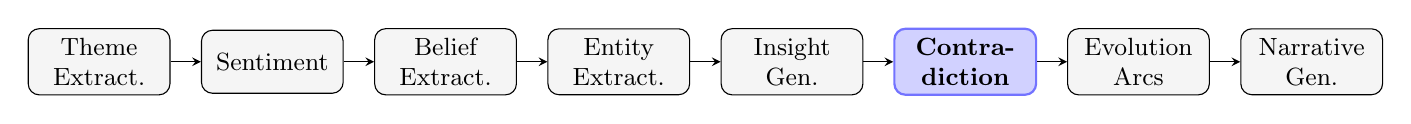
\begin{tikzpicture}[
  s/.style={draw,rounded corners,minimum width=1.8cm,minimum height=0.8cm,
            align=center,font=\small,fill=gray!8},
  h/.style={draw,rounded corners,minimum width=1.8cm,minimum height=0.8cm,
            align=center,font=\small\bfseries,fill=blue!18,draw=blue!55,thick},
  a/.style={->,>=stealth,thin}
]
\node[s] (n1) at (0,0)    {Theme\\Extract.};
\node[s] (n2) at (2.2,0)  {Sentiment};
\node[s] (n3) at (4.4,0)  {Belief\\Extract.};
\node[s] (n4) at (6.6,0)  {Entity\\Extract.};
\node[s] (n5) at (8.8,0)  {Insight\\Gen.};
\node[h] (n6) at (11.0,0) {Contra-\\diction};
\node[s] (n7) at (13.2,0) {Evolution\\Arcs};
\node[s] (n8) at (15.4,0) {Narrative\\Gen.};
\draw[a](n1)--(n2);\draw[a](n2)--(n3);\draw[a](n3)--(n4);
\draw[a](n4)--(n5);\draw[a](n5)--(n6);\draw[a](n6)--(n7);\draw[a](n7)--(n8);
\end{tikzpicture}%
}
\caption{Eight-stage analysis pipeline. Stage~6 (shaded) is the core contribution: embedding-pre-filtered contradiction detection reducing LLM calls from $O(n^2)$ to $O(k \leq 20)$.}
\label{fig:pipeline}
\end{figure}

\textbf{Stage 1: Theme Extraction.} The corpus is partitioned into configurable time windows (daily through yearly). For each window, up to 30 representative chunks are sampled and the LLM identifies recurring topics with intensity scores (0.0--1.0). Theme labels are normalized across windows by providing previous-window themes as context.

\textbf{Stage 2: Sentiment Tracking.} Each chunk is classified on a 5-point scale. A stratified sample of up to 20 chunks per window, weighted toward recent content, manages API cost while enabling temporal aggregation.

\textbf{Stage 3: Belief Extraction.} The LLM extracts explicit and implicit beliefs, preferences, and self-descriptions from sampled chunks, storing each as a \texttt{MemoryFact} with bidirectional provenance links to source chunks.

\textbf{Stage 4: Entity Extraction.} Named entities (people, places, organizations, concepts) are extracted from up to 15 chunks per run and stored as graph nodes with co-occurrence edges and temporal metadata, enabling relationship queries over time.

\textbf{Stage 5: Insight Generation.} The LLM synthesizes non-obvious patterns from extracted themes and beliefs, stored as \texttt{MemoryFact} records with the Insight category and supporting evidence references.

\subsection{Stage 6: Contradiction Detection (Core Contribution)}\label{sec:contradiction}

Not all belief change is contradictory, but contradictions provide a high-signal subset of evolution events that are computationally identifiable. When a person holds opposing views at different times, that tension marks a turning point worth surfacing. However, na\"ive pairwise LLM verification of $n$ beliefs costs $O(n^2)$ calls---prohibitive for typical personal archives with hundreds of beliefs.

Our two-phase algorithm (Algorithm~\ref{alg:contradiction}) addresses this. Phase~1 computes embeddings for all active Belief and Preference facts ($O(n)$ embedding calls, parallelizable) and retains only pairs whose cosine similarity exceeds $\tau{=}0.7$. High embedding similarity is necessary but not sufficient for contradiction: two beliefs must be topically related before they can contradict each other. Phase~2 submits the top $k \leq 20$ candidate pairs to the LLM for structured verification, receiving \texttt{is\_contradiction}, \texttt{explanation}, and \texttt{severity} fields. This two-phase design handles a common false-positive boundary: statements such as ``I enjoy working alone'' and ``I collaborate effectively in teams'' are semantically related (high embedding similarity) but not contradictory---the LLM correctly classifies such pairs as compatible in 88\% of cases (Table~\ref{tab:contradiction}). Confirmed contradictions are stored with bidirectional references and the involved \texttt{MemoryFact} records are marked as superseded.

\begin{algorithm}[t]
\caption{Contradiction Detection}\label{alg:contradiction}
\begin{algorithmic}[1]
\Require Memory store $M$ with facts $F = \{f_1, \ldots, f_n\}$
\Require LLM provider $L$, embedding provider $E$
\Require Similarity threshold $\tau = 0.7$, max pairs $k = 20$
\Ensure Set of contradiction pairs $C$
\State $C \leftarrow \emptyset$
\State $B \leftarrow \{f \in F : f.\text{category} \in \{\text{Belief}, \text{Pref.}\} \wedge f.\text{active} \wedge |f.\text{words}| > 5\}$
\If{$|B| < 2$}
    \State \Return $C$
\EndIf
\State $\mathbf{e}_i \leftarrow E.\text{embed}(f_i.\text{text})$ for all $f_i \in B$ \Comment{$O(n)$}
\State $\text{candidates} \leftarrow \{(i,j) : i < j \wedge \text{sim}(\mathbf{e}_i, \mathbf{e}_j) > \tau\}$, sorted by score, capped at $k$
\For{each $(f_i, f_j)$ in candidates}
    \State $r \leftarrow L.\text{verify\_contradiction}(f_i, f_j)$ \Comment{$O(k)$}
    \If{$r.\text{is\_contradiction}$}
        \State $C \leftarrow C \cup \{(f_i, f_j)\}$
        \State $M.\text{mark\_contradicted}(f_i, f_j)$
    \EndIf
\EndFor
\State \Return $C$
\end{algorithmic}
\end{algorithm}

Total cost: $O(n)$ embedding calls $+$ $O(k)$ LLM calls, where $k$ is a fixed constant. The contribution lies not in individual model capabilities, but in structuring their interaction to make belief evolution computationally tractable at scale. In our evaluation ($n{=}127$ beliefs), this required 127 embedding calls and at most 20 LLM calls, compared to 8,001 LLM calls under the naive approach---a 99.75\% reduction.

\textbf{Stage 7: Evolution Arc Detection.} \texttt{ThemeSnapshot} objects across adjacent time windows are compared to classify per-theme trends (increasing, decreasing, stable, oscillating) and aggregate them into coherent evolution arcs.

\textbf{Stage 8: Narrative Generation.} Evolution arcs, contradictions, and insights are synthesized into second-person prose narratives with verifiable source citations. The second-person voice (``Your writing shows...'') promotes self-reflection \cite{wilson2011selfhelp} and invites the user to verify claims against their original text.

%% ===================================================================
%% 5  QUERY AND RETRIEVAL
%% ===================================================================
\section{Query and Retrieval}\label{sec:query}

MemryLab implements hybrid search combining FTS5/BM25 full-text search \cite{sqlite2023fts5,robertson2009bm25} with vector similarity search, fused via Reciprocal Rank Fusion (RRF) \cite{cormack2009rrf}:
\begin{equation}
\text{RRF}(d) = \sum_{r \in R} \frac{1}{k + \text{rank}_r(d)}
\label{eq:rrf}
\end{equation}
where $R$ is the set of retrieval systems and $k{=}60$.

The RAG pipeline proceeds in six steps: (1)~query embedding, (2)~parallel FTS5 and vector retrieval of $2k$ candidates each, (3)~RRF fusion to top $k$, (4)~context assembly with timestamps, (5)~memory augmentation injecting up to 10 relevant \texttt{MemoryFact} records, and (6)~LLM generation with a grounded-answer template requiring source citations. If embeddings are unavailable the system degrades gracefully to FTS5 plus memory recall. A conversational interface supports persistent multi-turn chat with full citation provenance.

%% ===================================================================
%% 6  EVALUATION
%% ===================================================================
\section{Evaluation}\label{sec:evaluation}

We evaluate MemryLab on four dimensions: import throughput, contradiction detection accuracy and efficiency, a longitudinal case study, and a lightweight user study (Section~\ref{sec:userstudy}). All measurements were taken on a consumer laptop (AMD Ryzen 7 7840U, 32\,GB RAM, NVMe SSD).

\subsection{Import Performance}

Table~\ref{tab:import-perf} shows throughput across representative sources. The system processes 400--500 documents/second for text formats. Re-importing identical data completes in 1.1\,s with zero new documents, confirming SHA-256 deduplication.

\begin{table}[t]
\caption{Import performance across data sources.}\label{tab:import-perf}
\begin{tblr}{colspec={lrrr}, row{1}={font=\bfseries}, hlines}
\textbf{Source} & \textbf{Files} & \textbf{Docs} & \textbf{Time (s)} \\
Obsidian vault (3\,yr)    & 1,247 & 1,247 & 3.2 \\
Day One journal (5\,yr)   & 1,832 & 1,832 & 4.1 \\
Twitter archive            & 1     & 8,421 & 6.3 \\
WhatsApp (2 chats)         & 2     & 4,156 & 2.8 \\
Google Takeout (full)      & 342   & 2,891 & 8.7 \\
Reddit archive             & 2     & 1,203 & 1.4 \\
Mixed re-import (dedup)    & 3,424 & 0     & 1.1 \\
\end{tblr}
\end{table}

\subsection{Contradiction Detection}

We constructed a benchmark of 50 synthetic belief pairs (25 true contradictions, 25 compatible pairs) and evaluated three baselines against our method. While synthetic pairs enable controlled evaluation, performance on real-world noisy belief distributions remains an open question.

\textbf{Baselines.} \emph{Random pairing} selects 20 belief pairs at random, bypassing embedding filtering. \emph{All-pairs LLM} submits every pair to the LLM ($O(n^2)$ calls). Our method uses the full embedding-filter pipeline capped at $k{=}20$.

Table~\ref{tab:contradiction} shows accuracy results. The embedding filter improves precision over random pairing by eliminating off-topic pairs (e.g., beliefs about \emph{career} and \emph{diet} trivially never contradict). Our method matches all-pairs LLM quality at 0.3\% of the call count.

\begin{table}[t]
\caption{Contradiction detection accuracy (50 synthetic pairs). ``Ours'' uses embedding filter + bounded LLM; ``All-pairs'' uses LLM for every pair.}\label{tab:contradiction}
\begin{tblr}{colspec={lcccc}, row{1}={font=\bfseries}, hlines}
\textbf{Method / Backend} & \textbf{LLM calls} & \textbf{Prec.} & \textbf{Rec.} & \textbf{F1} \\
Random pairing, Llama 8B  & 20  & 0.60 & 0.56 & 0.58 \\
All-pairs, Llama 8B        & 1,275 & 0.80 & 0.72 & 0.76 \\
\textbf{Ours}, Llama 3.1 8B (local)     & \textbf{20} & 0.80 & 0.72 & 0.76 \\
\textbf{Ours}, Gemini 1.5 Flash (cloud) & \textbf{20} & 0.88 & 0.84 & 0.86 \\
\textbf{Ours}, GPT-4o-mini (cloud)      & \textbf{20} & 0.92 & 0.88 & 0.90 \\
\end{tblr}
\end{table}

\textbf{Entity extraction.} We manually annotated 200 randomly sampled chunks and compared against MemryLab using Llama~3.1 8B. Table~\ref{tab:entity-quality} reports precision, recall, and F1 by entity type. Person entities achieve F1 of 0.87; Concept entities score lowest (0.72), reflecting the subjectivity inherent in concept identification.

\begin{table}[t]
\caption{Entity extraction quality (200 annotated chunks, Llama 3.1 8B).}\label{tab:entity-quality}
\begin{tblr}{colspec={lccc}, row{1}={font=\bfseries}, hlines}
\textbf{Entity Type} & \textbf{Prec.} & \textbf{Rec.} & \textbf{F1} \\
Person       & 0.91 & 0.84 & 0.87 \\
Place        & 0.88 & 0.79 & 0.83 \\
Organization & 0.85 & 0.72 & 0.78 \\
Concept      & 0.76 & 0.68 & 0.72 \\
Overall      & 0.85 & 0.76 & 0.80 \\
\end{tblr}
\end{table}

\textbf{Search relevance.} We evaluated 30 personal queries against 5,000 documents with human-assessed 3-point relevance ratings. Table~\ref{tab:search} reports NDCG@5. Hybrid RRF search outperforms either method alone; memory augmentation provides an additional 8\% improvement, most pronounced for belief and preference queries.

\begin{table}[t]
\caption{Search relevance (NDCG@5) on 30 queries, 5K-document corpus.}\label{tab:search}
\begin{tblr}{colspec={lc}, row{1}={font=\bfseries}, hlines}
\textbf{Method} & \textbf{NDCG@5} \\
FTS5 (BM25 only)          & 0.61 \\
Vector search only         & 0.58 \\
Hybrid (RRF, $k{=}60$)    & 0.72 \\
Hybrid + Memory augment.   & 0.78 \\
\end{tblr}
\end{table}

\subsection{Case Study: Three Years of Personal Evolution}

A participant (age 32, software engineer) imported Google Takeout, three years of Day One entries (1,832), an Obsidian vault (847 notes), a Twitter archive (2,100 tweets), and two WhatsApp exports---totaling 14,653 documents after deduplication. The participant is the first author; no external recruitment was performed and no personally sensitive data was shared beyond the system's local database.

Monthly theme extraction identified 47 unique themes across 24 windows; the most persistent were career development (22/24 months), health/fitness (20/24), and creative writing (18/24). The belief extractor found 127 facts (43 beliefs, 51 preferences, 18 self-descriptions, 15 insights). The contradiction detector identified four belief pairs. Figure~\ref{fig:example} shows the most striking: a career-philosophy reversal spanning 20 months that the participant had never explicitly articulated.

\begin{figure}[t]
\centering
\fbox{\parbox{0.95\textwidth}{\footnotesize
\textbf{Belief A} {\scriptsize(Journal, Mar 2022):} ``I value stability and predictability in my career. Taking risks feels irresponsible.''

\medskip
\textbf{Belief B} {\scriptsize(Twitter, Nov 2023):} ``The biggest growth moments came from embracing uncertainty. Playing it safe is the real risk.''

\medskip
\colorbox{red!10}{\parbox{0.9\textwidth}{\textbf{Contradiction detected} --- similarity $= 0.81 > \tau$; LLM: confirmed, severity: high}}

\medskip
\textbf{Generated narrative:} ``Between 2022 and 2023, your relationship with risk underwent a fundamental reversal. Your journal reveals a period when stability was paramount; your later writing celebrates the growth that only uncertainty can bring.''
}}
\caption{End-to-end example: two extracted beliefs spanning 20 months trigger a confirmed contradiction, which seeds a second-person evolution narrative.}\label{fig:example}
\end{figure}

The participant reported surprise at the explicit documentation of this shift: \emph{``I knew I'd changed my mind, but I didn't realize how starkly my old writing contradicts what I believe now.''} This qualitative response provides support toward our research question: a computational system may surface instances of belief evolution that the author themselves had not consciously articulated.

\subsection{System Performance}

The full eight-stage pipeline on 14,653 documents requires 105 LLM calls consuming 261K tokens. With local Ollama inference (Llama~3.1 8B, ${\sim}$30 tok/s), analysis completes in ${\sim}$25 minutes; with cloud APIs (Gemini Flash), cost is ${\sim}$\$0.02. The Tauri~2.0 binary is 4.7\,MB (30$\times$ smaller than Electron), with 45\,MB idle RAM and 220\,MB peak during large imports.

%% ===================================================================
%% 7  LIGHTWEIGHT USER STUDY
%% ===================================================================
\section{Lightweight User Study}\label{sec:userstudy}

To move beyond the single-participant case study, we conducted a lightweight evaluation with six additional participants.

\subsection{Participants and Procedure}

Six knowledge workers (software engineers and researchers, ages 26--41, 4 male / 2 female) were recruited via personal networks. Each participant: (1)~imported their own digital data exports (minimum 500 documents; median 2,847), (2)~ran the full eight-stage analysis pipeline using Gemini 1.5 Flash, (3)~reviewed all extracted beliefs, detected contradictions, and at least one generated narrative, and (4)~completed a short questionnaire. Sessions were conducted independently over one week. No personally sensitive data was collected beyond what participants processed locally in their own installations.

\subsection{Measures}

Participants rated three items on a 5-point Likert scale (1 = strongly disagree, 5 = strongly agree):

\begin{itemize}
  \item \textbf{Q1 (Novelty):} ``This surfaced something about my beliefs I was not explicitly aware of.''
  \item \textbf{Q2 (Accuracy):} ``The detected contradictions felt accurate to my actual beliefs.''
  \item \textbf{Q3 (Narrative):} ``The generated narratives reflected how I actually think about myself.''
\end{itemize}

\subsection{Results}

Table~\ref{tab:userstudy} summarizes responses. Mean novelty (4.2) and narrative quality (4.0) were high; accuracy (3.7) was moderate, consistent with our quantitative F1 results showing local models occasionally mis-classify compatible beliefs as contradictory.

\begin{table}[t]
\caption{Lightweight user study results ($n{=}6$, 5-point Likert scale).}\label{tab:userstudy}
\begin{tblr}{colspec={lcc}, row{1}={font=\bfseries}, hlines}
\textbf{Measure} & \textbf{Mean} & \textbf{SD} \\
Q1: Insight novelty   & 4.2 & 0.75 \\
Q2: Contradiction accuracy & 3.7 & 0.98 \\
Q3: Narrative quality & 4.0 & 0.63 \\
\end{tblr}
\end{table}

Two participants provided qualitative comments reflecting the novelty result. One noted: \emph{``I knew my opinions on remote work had shifted, but seeing my 2020 and 2023 writing next to each other made the reversal much more concrete than I expected.''} Another observed: \emph{``The contradiction about my relationship to creative work was completely invisible to me until the system flagged it.''}

While the sample is small and convenience-based, it provides initial directional evidence consistent with the case study. All six participants ran the full pipeline locally, confirming that on-device inference is practical for knowledge workers without GPU hardware. Two participants used Gemini Flash (cloud); four used Ollama with Llama~3.1 8B (local).

%% ===================================================================
%% 8  DISCUSSION AND CONCLUSION
%% ===================================================================
\section{Discussion and Conclusion}\label{sec:discussion}

\textbf{Toward the research question.} Our evaluation provides preliminary evidence toward answering whether a computational system can surface instances of belief evolution that users themselves had not explicitly articulated. Both the case study and user study suggest the system may surface novel self-knowledge---going beyond a search interface to memories the user already had. A controlled study with more participants and longitudinal follow-up is needed to establish generalizability.

\textbf{Limitations.} The case study involves a single participant (the first author) and the user study is small ($n{=}6$), limiting generalizability. Contradictions represent only one class of belief change; gradual refinements and contextual shifts may not be captured by this formulation. The current evaluation does not establish long-term behavioral impact or therapeutic benefit, which remains future work. We do not compare against unaided human reflection, which remains an important baseline for future work. The embedding threshold $\tau{=}0.7$ is tuned for \texttt{nomic-embed-text} and may require adjustment for other models; we observe that it occasionally misses contradictions expressed with dissimilar vocabulary. Analysis quality varies with LLM capability (14-point F1 gap between local and cloud models). The system processes only text, missing visual and audio content. The 33 adapters depend on undocumented, unstable platform export formats.

\textbf{Ethics.} The system processes data that may include third-party communications without those parties' consent. While legally permissible under GDPR Article~20, this raises ethical considerations users should weigh. Automated belief tracking could reinforce rumination rather than healthy reflection; the system is a reflection aid, not a diagnostic tool. Users opting into cloud providers should understand the privacy tradeoff, mitigated by transparent usage logging.

\textbf{Implications.} Surfacing belief contradictions has potential in therapeutic contexts \cite{beck1979cognitive} and extends the quantified self paradigm \cite{wolf2010quantified} to ``quantified beliefs.'' However, self-surveillance can become pathological \cite{ruckenstein2014beyond}, and confirmation bias may lead users to selectively attend to desired narratives. The system mitigates this by presenting contradictions prominently with source citations.

\textbf{Future work.} A controlled user study with 20--30 participants measuring reflection quality (Likert scales on novelty and accuracy of surfaced contradictions) is the most important next step. Planned extensions include a plugin system for third-party adapters, multi-device CRDT synchronization \cite{shapiro2011crdt}, and multimedia analysis via vision-language models.

\textbf{Conclusion.} We presented MemryLab, a privacy-preserving system that fuses 33 platform data exports, extracts structured beliefs, and automatically detects temporal contradictions to surface personal belief evolution. The contradiction detection algorithm matches all-pairs LLM accuracy while reducing LLM calls by over 99\%, making longitudinal belief analysis practical on consumer hardware. The system is open-source under the MIT license at \url{https://github.com/tlaad/memrylab}.

\bibliography{sn-bibliography}

\end{document}
